\setcounter{figure}{0} 
\setcounter{table}{0}
\setcounter{footnote}{0}
\setcounter{equation}{0}
\pagestyle{fancy}
\fancyhf{}
\renewcommand{\chaptermark}[1]{\markboth{\MakeUppercase{#1 }}{}}
\renewcommand{\sectionmark}[1]{\markright{\thesection~ #1}}
\fancyhead[RO]{\bfseries\rightmark}
\fancyhead[LE]{\bfseries\leftmark}
\fancyfoot[RO]{\thepage}
\fancyfoot[LE]{\thepage}
\renewcommand{\headrulewidth}{0.5pt}
\renewcommand{\footrulewidth}{0pt}

\makeatletter
\renewcommand\thefigure{D.\arabic{figure}}
\renewcommand\thetable{D.\arabic{table}} 
\makeatother

\chapter{Annexe D : Solution Mantis VW}
\graphicspath{{Annexe4/figures/}}
%==========================================================================

%    Annexe

%===========================================================================
\begin{figure}[!ht]\centering
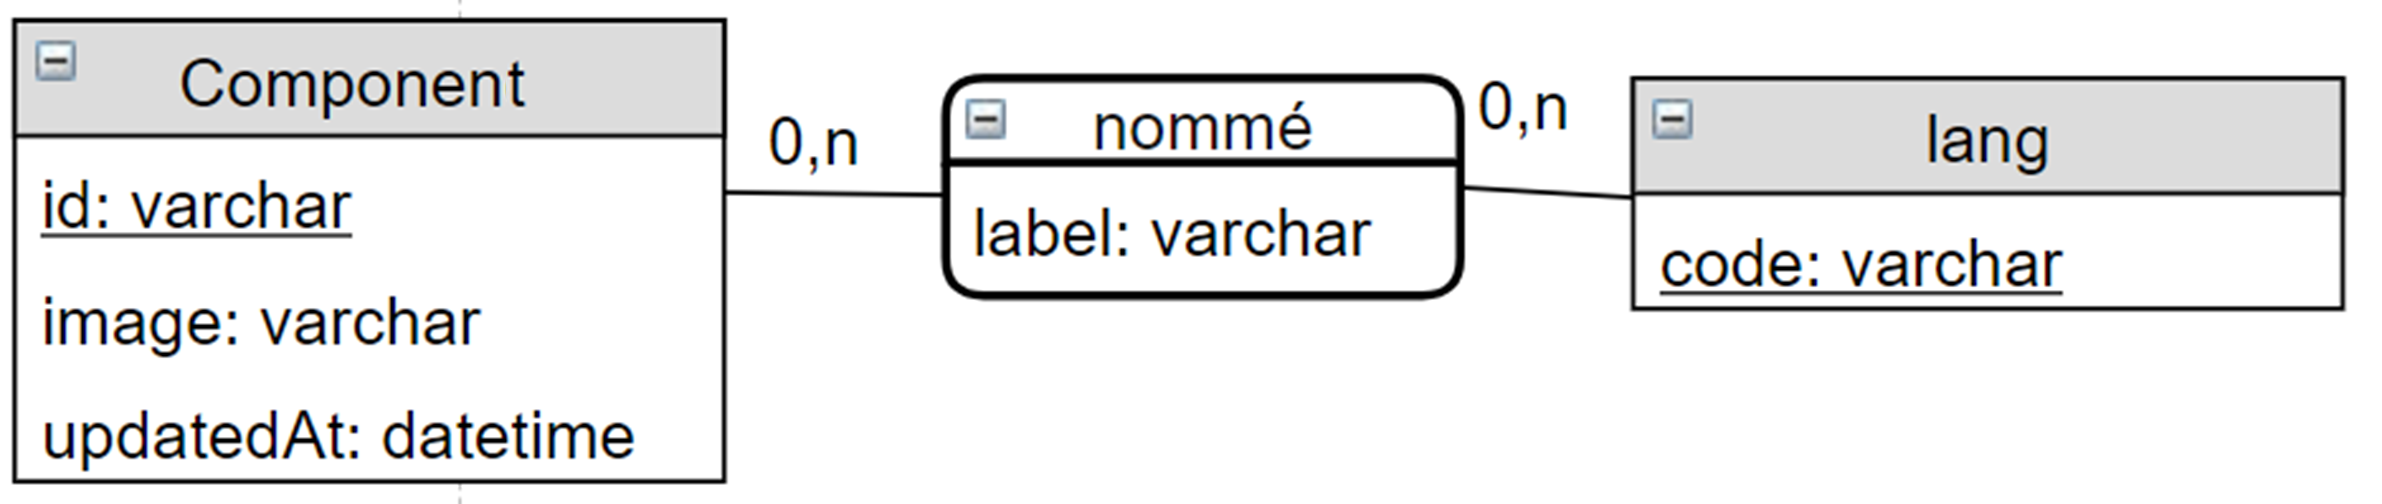
\includegraphics[scale=0.15]{mcd2.png}
\caption{Modèle conceptuel des données pour l'internationalisation}
\label{fig:fig1}
\end{figure}
\FloatBarrier
\begin{figure}[!ht]\centering
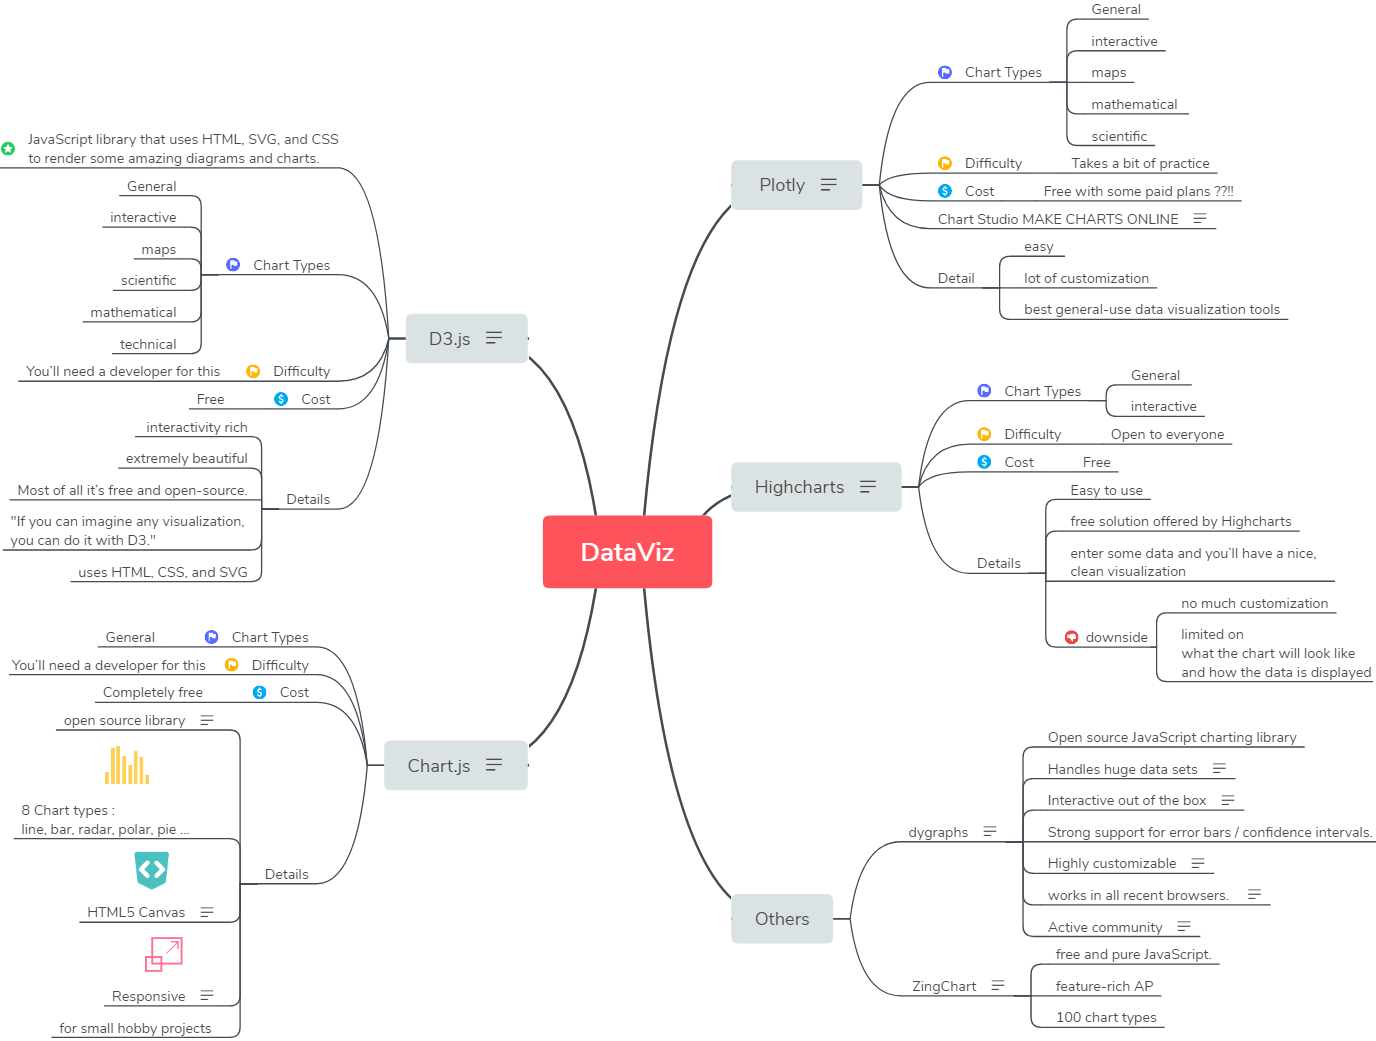
\includegraphics[scale=0.4]{DataViz.png}
\caption{Map de comparaison entre des biothèques JavaScript de visualisation des sonnées}
\label{fig:fig1}
\end{figure}
\FloatBarrier

\begin{itemize}
\item[D.1.] Le modèle MVC a été présenté par de nombreux développeurs comme un modèle utile pour la réutilisation du code objet et un modèle qui leur permet d’augmenter la productivité des développeurs des applications. Il propose trois composants ou objets principaux à utiliser dans le développement de logiciels :
    \begin{itemize}
    \item[--] Un modèle, qui représente la structure logique sous-jacente des données dans une application logicielle et la classe de haut niveau qui lui est associée. Ce modèle d'objet ne contient aucune information sur l'interface utilisateur.
    \item[--] Une vue, qui est une collection de classes représentant les éléments de l'interface utilisateur (toutes les choses que l'utilisateur peut voir et auxquelles il peut répondre à l'écran, telles que les boutons, les zones d'affichage, etc.).
    \item[--] Un contrôleur, qui représente les classes connectant le modèle et la vue, permet de communiquer entre les classes du modèle et de la vue.
    \end{itemize}
\end{itemize}
\begin{figure}[!ht]\centering
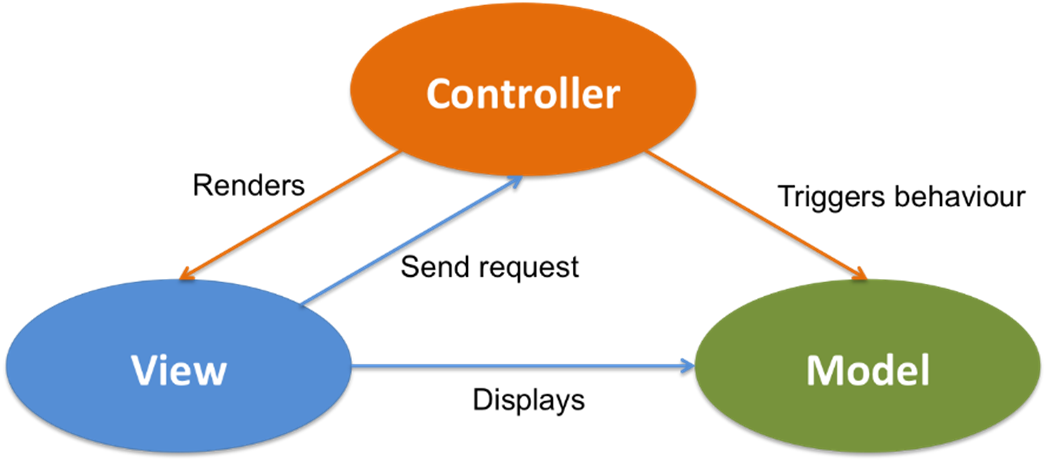
\includegraphics[scale=0.4]{mvc.png}
\caption{Modèle MVC \cite{mvc}}
\label{fig:fig1}
\end{figure}
\FloatBarrier
\begin{itemize}
\item[D.2.] Le BDD (Behavior Driven Development) est une approche collaborative du développement agile qui comble le manque de communication entre les experts métiers et l’équipe de développement. BDD aide les équipes à communiquer les exigences avec plus de précision, à détecter rapidement les défauts et à produire des logiciels qui restent maintenables au fil du temps. Cela aide les équipes à créer des exigences métier compréhensibles et conduit à moins de retouches et à une mise sur le marché plus rapide.
\item[D.3.] Test Driven Development (TDD) est une pratique de programmation qui demande aux développeurs d'écrire du nouveau code uniquement si un test automatisé a échoué. Cela évite la duplication du code. L’objectif principal de TDD est de rendre le code plus clair, simple et sans bug. Dans une approche TDD le test est développé pour spécifier et valider ce que fera le code.
\end{itemize}
